\documentclass[conference]{IEEEtran}
\IEEEoverridecommandlockouts

\usepackage{cite}
\usepackage{amsmath,amssymb}
\usepackage{graphicx}
\usepackage{booktabs}
\usepackage{url}

\begin{document}

\title{Robustness of XAI Explanations Under Adversarial Noise}

\author{
\IEEEauthorblockN{Your Name}
\IEEEauthorblockA{
Department of Computer Science\\
Your University\\
City, Country\\
email@domain.com}
}

\maketitle

\begin{abstract}
Explainable AI methods are commonly used to interpret deep neural networks, but their reliability under adversarial perturbations remains unclear. This paper evaluates the robustness of Grad-CAM explanations under Fast Gradient Sign Method (FGSM) attacks on CIFAR-10. A ResNet-18 classifier is trained on CIFAR-10 and then evaluated by comparing Grad-CAM maps generated from clean and adversarial inputs. Explanation drift is quantified using cosine similarity, while predictive robustness is measured using attack success rate. Across three seeds, the model achieves average test accuracy of 0.7852 $\pm$ 0.0059, mean Grad-CAM cosine similarity of 0.7315 $\pm$ 0.0510, and FGSM attack success rate of 0.8967 $\pm$ 0.0153 at $\epsilon=0.02$. Results indicate moderate average explanation stability with high sample-level variance, showing that explanation robustness is context-dependent and should be evaluated statistically.
\end{abstract}

\begin{IEEEkeywords}
Explainable AI, Grad-CAM, Adversarial Attacks, FGSM, Robustness, CIFAR-10, ResNet-18
\end{IEEEkeywords}

\section{Introduction}
Deep neural networks provide high classification accuracy, but their decision process is difficult to interpret. Post-hoc explainability tools such as Grad-CAM are often used to highlight regions that contribute to model predictions. At the same time, adversarial examples can alter predictions using small perturbations that are often imperceptible to humans. This leads to an important reliability question: do visual explanations remain stable when adversarial perturbations are applied?

This work studies the robustness of Grad-CAM under FGSM perturbations for CIFAR-10 classification. Instead of relying on isolated case studies, we evaluate explanation drift over multiple random samples and seeds. The pipeline reports both predictive vulnerability and explanation shift, providing a clearer view of model trustworthiness under adversarial conditions.

\section{Related Work}
Goodfellow \emph{et al.} introduced FGSM as an efficient single-step attack based on input gradient sign \cite{goodfellow2015}. Selvaraju \emph{et al.} proposed Grad-CAM, a class-discriminative localization method for CNN explanations \cite{selvaraju2017}. Residual networks are widely used for robust visual classification benchmarks \cite{he2016}. CIFAR-10 is a standard compact dataset for controlled computer vision experiments \cite{krizhevsky2009}.

\section{Methodology}
\subsection{Dataset and Model}
The dataset is CIFAR-10, containing 60,000 RGB images of size $32\times32$ across 10 classes. A ResNet-18 architecture is adapted with a 10-class output head and trained from scratch. Input normalization is embedded in the network using CIFAR-10 mean and standard deviation.

\subsection{Adversarial Perturbation}
Given an image $x$, FGSM generates an adversarial example:
\begin{equation}
    x_{adv}=\text{clip}\left(x+\epsilon\cdot\text{sign}(\nabla_x J(\theta,x,y)),0,1\right)
\end{equation}
where $\epsilon$ controls perturbation magnitude.

\subsection{Explanation Robustness Metric}
For each sampled image, Grad-CAM is generated for both clean and adversarial inputs with the clean predicted class as target. Explanation drift is measured using cosine similarity:
\begin{equation}
\text{CosSim}(A,B)=\frac{A\cdot B}{\|A\|_2\|B\|_2}
\end{equation}
where $A$ and $B$ are flattened clean and adversarial saliency maps.

\subsection{Evaluation Pipeline}
The workflow is:
\begin{enumerate}
\item Predict class on clean input.
\item Generate clean Grad-CAM.
\item Generate FGSM adversarial input.
\item Predict class on adversarial input.
\item Generate adversarial Grad-CAM.
\item Compute cosine similarity and attack success indicator.
\end{enumerate}

Aggregate metrics reported are mean, standard deviation, minimum, and maximum cosine similarity, plus attack success rate.

\section{Experimental Setup}
Training uses SGD with momentum 0.9, weight decay $5\times10^{-4}$, and cosine annealing schedule for 10 epochs. Data augmentation includes random crop and random horizontal flip. Evaluation is run with $\epsilon=0.02$ using 100 random test samples per seed for seeds 42, 7, and 123.

\section{Results}
\subsection{Quantitative Results}
Table \ref{tab:results} summarizes per-seed results.

\begin{table}[htbp]
\caption{Per-seed robustness results ($\epsilon=0.02$)}
\label{tab:results}
\centering
\begin{tabular}{ccccc}
\toprule
Seed & Test Acc & Mean CosSim & CosSim Std & Attack SR \\
\midrule
42  & 0.7788 & 0.7324 & 0.3638 & 0.8800 \\
7   & 0.7905 & 0.6801 & 0.3904 & 0.9000 \\
123 & 0.7862 & 0.7820 & 0.2469 & 0.9100 \\
\bottomrule
\end{tabular}
\end{table}

Cross-seed averages are: test accuracy 0.7852 $\pm$ 0.0059, mean cosine similarity 0.7315 $\pm$ 0.0510, and attack success rate 0.8967 $\pm$ 0.0153.

These numbers show high adversarial vulnerability and moderate explanation stability on average, with strong variance across samples.

\subsection{Qualitative Analysis with Figures}
Figure \ref{fig:qual0} and Figure \ref{fig:qual1} compare clean and adversarial cases. In each row, the order is: clean image, adversarial image, clean Grad-CAM, adversarial Grad-CAM.

\begin{figure*}[htbp]
\centering
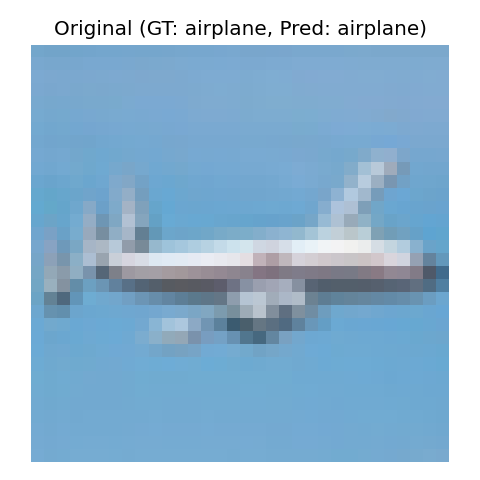
\includegraphics[width=0.24\textwidth]{figures/sample_000_original.png}
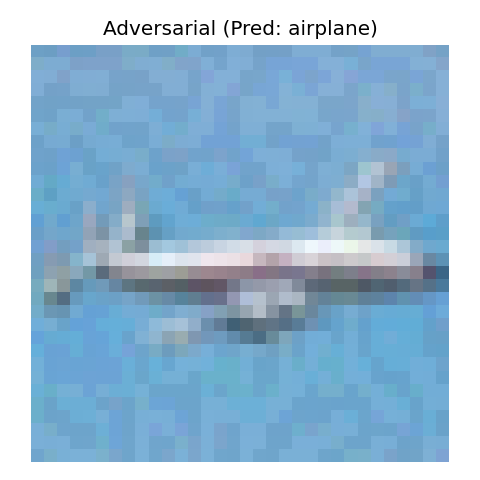
\includegraphics[width=0.24\textwidth]{figures/sample_000_adversarial.png}
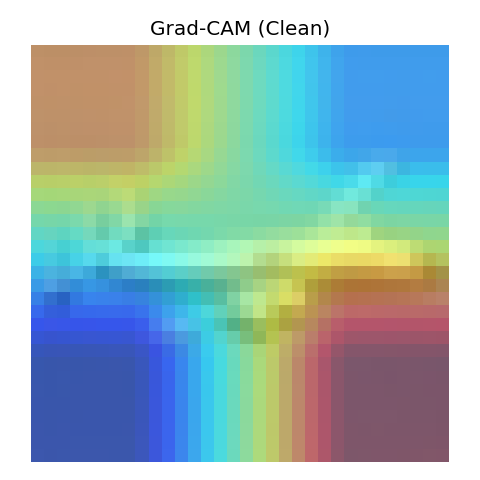
\includegraphics[width=0.24\textwidth]{figures/sample_000_gradcam_clean.png}
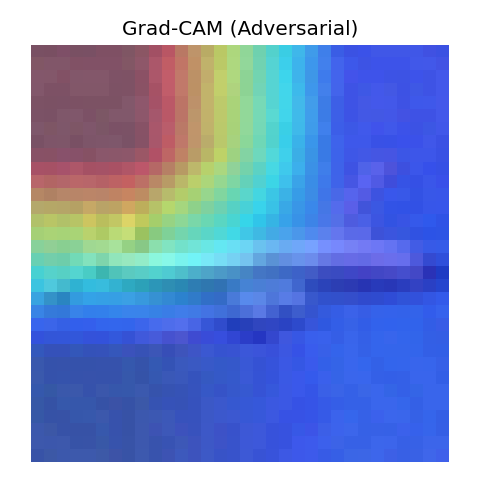
\includegraphics[width=0.24\textwidth]{figures/sample_000_gradcam_adversarial.png}
\caption{Sample 000: clean and adversarial comparison with Grad-CAM overlays.}
\label{fig:qual0}
\end{figure*}

\begin{figure*}[htbp]
\centering
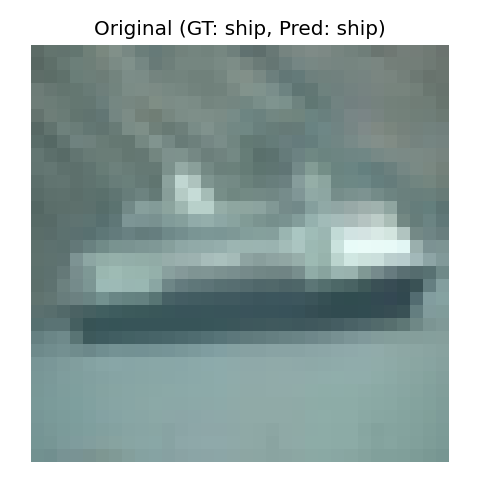
\includegraphics[width=0.24\textwidth]{figures/sample_001_original.png}
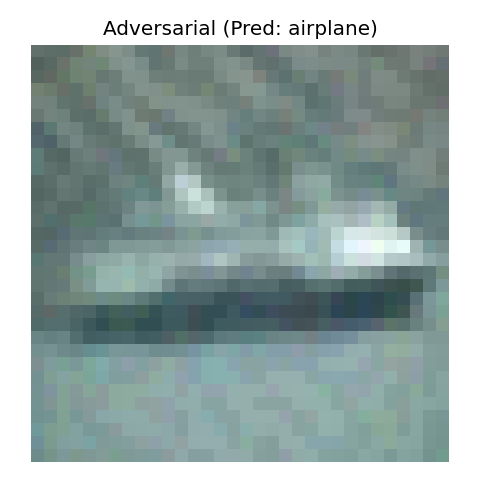
\includegraphics[width=0.24\textwidth]{figures/sample_001_adversarial.png}
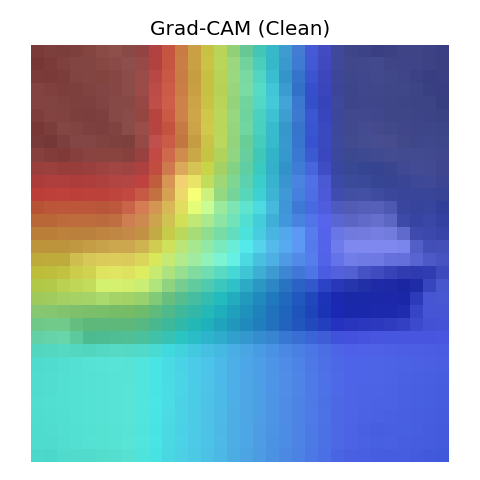
\includegraphics[width=0.24\textwidth]{figures/sample_001_gradcam_clean.png}
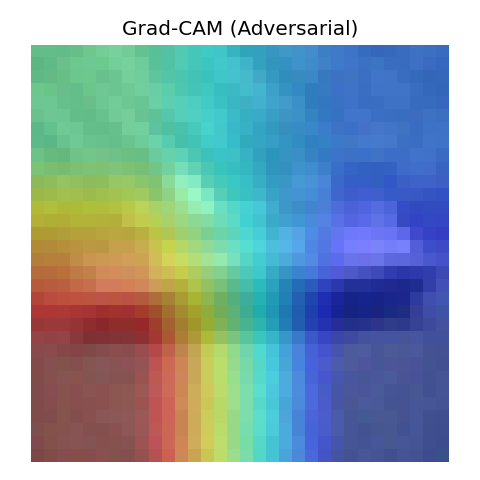
\includegraphics[width=0.24\textwidth]{figures/sample_001_gradcam_adversarial.png}
\caption{Sample 001: clean and adversarial comparison with Grad-CAM overlays.}
\label{fig:qual1}
\end{figure*}

Both examples demonstrate explanation drift after perturbation. In some cases, class prediction changes with clear saliency relocation; in others, prediction can remain stable while attention focus still shifts.

\section{Discussion}
The experiments suggest that prediction robustness and explanation robustness are related but not equivalent. High attack success confirms model fragility, while cosine similarity distribution shows that explanation drift is uneven across inputs. Therefore, a reliable XAI robustness study should report distributions and not only a few visual examples.

\section{Limitations and Future Work}
This study evaluates a single attack (FGSM) and one explanation method (Grad-CAM). Future work should include iterative attacks (for example, PGD), stronger model baselines, and additional explanation methods to assess whether observed trends generalize.

\section{Conclusion}
This paper presented an IEEE-style reproducible study of Grad-CAM robustness under adversarial noise on CIFAR-10. Results show that explanations are moderately stable on average but significantly variable across samples, and model predictions are highly vulnerable to FGSM. These findings support statistically grounded evaluation of XAI reliability.

\bibliographystyle{IEEEtran}
\bibliography{references}

\end{document}
